The simple corner detectors like Harris (section~\ref{subsec:harris-corner-detection}) can work only when the images are similar in  nature (same scale, orientation, intensity etc)~\cite{Lowe:04}. The SIFT features are invariant to image scaling and rotation, and partially invariant to change in illumination and 3D camera viewpoint. The features are highly distinctive ensuring a single feature to be correctly matched with high probability against a large database of features, thus making it applicable to image registration~\cite{Lowe:04}. \\ 

\noindent SIFT features detection consists of following steps:
\begin{enumerate}
	\item \textbf{Scale-space extrema detection:} This step finds out the potential interest points which are invariant to scale and orientation. This is carried out by using a difference of Gaussian (DoG) function. Extreme points are searched over all scales and image locations. The \emph{Difference of Gaussian} function is convolved with the image to get DoG image $D(x,y,\sigma)$. Mathematically, this can be represented as follows: 

\begin{equation}
D(x,y,\sigma)=(G(x,y,k \sigma)-G(x,y,\sigma))*I(x,y) 
\label{eq:state-space-image}
\end{equation}
which is equivalent to 
\begin{equation}
D(x,y,\sigma)=L(x,y,k \sigma)-L(x,y, \sigma)
\label{eq:equiv-state-space}
\end{equation}
where $G(x,y,\sigma)$ is Gaussian function [equation~\ref{eq:gaussian-function}]. $k$ is constant multiplicative factor. The \emph{DoG} function is preferred to \emph{Laplacian of Gaussian (LoG)} because it is simple to compute and the result can be close approximation to LoG~\cite{Lowe:04}. David Lowe has derived the relationship of LoG and DoG images as:

\begin{equation}
G(x,y,k \sigma)-G(x,y, \sigma) \approx (k-1)\sigma^2 \Delta^2G
\label{eq:dog-log}
\end{equation}
which shows DoG and LoG are differed only by a constant factor $k-1$. \\

\noindent This stage consists of two processes:\\
\textit{Construction of DoG images} As shown in figure~\ref{fig:dog-const}, the initial image is incrementally convolved with Gaussians to produce images separated by a constant factor $k$ in scale space (the left column in the figure). The approximation error will be zero when $k$ is 1 and David Lowe in~\cite{Lowe:04} also claims the stability of extrema even with significant differences in scale even when $k=\sqrt{2}$. For each octave of scale space (doubling of $\sigma$),the top image is re-sampled by taking every second pixel in each row and column to create the initial image for next octave with double $\sigma$ which greatly simplifies the computation. The adjacent images in the stack of the octave are subtracted to produce the DoG images as shown in figure~\ref{fig:dog-const}.\\

\begin{figure}[H]%
\centering
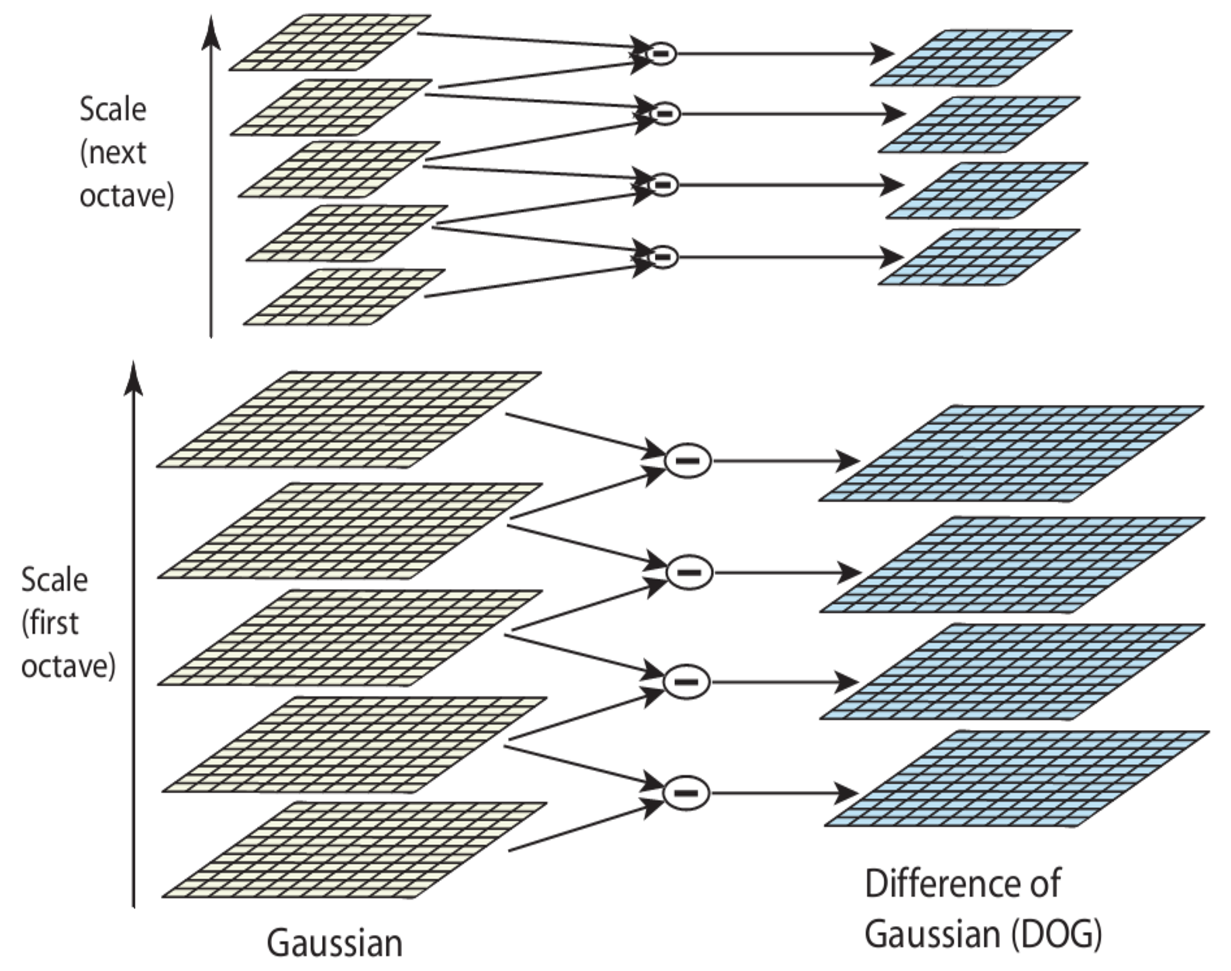
\includegraphics[width=0.9\columnwidth]{2.mainmatter/2.Methodology/FeaturesExtraction/figures/SIFT/difference-of-gaussian}%
\caption[Construction of DoG Image]{Construction of DoG image. \imgsrc{(Image source: Lowe~\cite{Lowe:04})}}%
\label{fig:dog-const}%
\end{figure}

\textit{Local extrema detection} As shown in figure~\ref{fig:max-min-dog}, the local maxima and minima of DoG images are found out by comparing each sample point to its eight neighbors in the current image and nine neighbors in the scale above and below. In 2D situation, we need to compare 3 DoG images in each octave, so we have to construct 4 different scale images~\cite{Li:11}.

\begin{figure}%
\centering
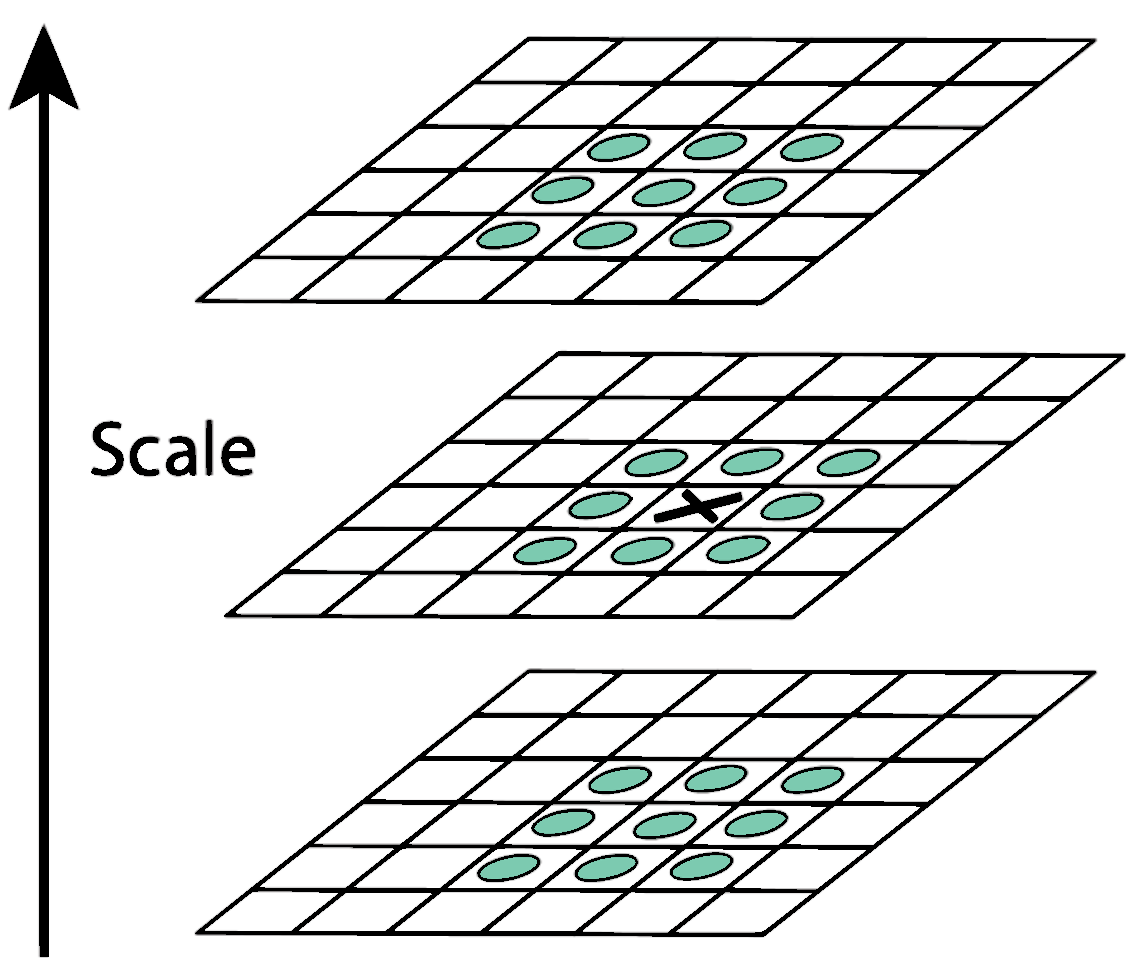
\includegraphics[width=0.6\columnwidth]{2.mainmatter/2.Methodology/FeaturesExtraction/figures/SIFT/maxima-minima-identification}%
\caption[Maxima and Minima of DoG Images]{Maxima and minima idenfication of DoG images. \imgsrc{(Image Source: Lowe~\cite{Lowe:04})}}%
\label{fig:max-min-dog}%
\end{figure}

\item \textbf{Key point localization:} This step performs a detailed fit to nearby data for location, scale, and ratio of principal curvatures so that we can remove the points with low contrast or poorly localized along the edge.\cite{Lowe:04}. To remove low contrast points, the magnitude of intensity is compared with a certain value, if it is less than the value, then reject it. Brown~\cite{Brown:02} suggested to use \emph{Taylor expansion} of the value at the extreme points to get the intensity. Similarly, to remove the edges, we use principal of Harris Corner Detector (section~\ref{subsec:harris-corner-detection}) i.e. in any point, if the ratio of largest magnitude eigenvalue and the smaller one is greater than some threshold, then it indicates the edge point. Suppose, $r$ is the threshold ratio of the two principal eigenvalues and $M$ is auto correlation matrix, we check the condition (modification of equation~\ref{eq:cornerness-map}):  
\begin{equation}
\frac{trace(M)^2}{det(M)}<\frac{(r+1)^2}{r}
\label{eq:edge-check}
\end{equation}

\item \textbf{Orientation assignment:} The orientation is assigned as key point descriptor so that we can achieve invariance to image rotation~\cite{Lowe:04}. Lowe suggests to use the following method for each key point to have stable results. The magnitude, $m(x,y)$ and orientation, $\theta(x,y)$  of the gradient is computed as:
\begin{equation}
m(x,y)=\sqrt{(L(x+1,y)-L(x-1,y))^2+(L(x,y+1)-L(x,y-1))^2}
\label{eq:orient-mag}
\end{equation}

\begin{equation}
\theta(x,y)=\tan^{-1}\frac{L(x,y+1)-L(x,y-1)}{L(x+1,y)-L(x-1,y)}
\label{eq:orient-theta}
\end{equation}
Lowe suggests to form an \emph{orientation histogram} from the gradient orientations of sample points withing a region around a key point and detect the highest peak. Any other local peak that is within 80\% of the highest peak is used to also create a key point with that orientation. So, for locations with multiple peaks of similar magnitude, there will be multiple key points created at the same location and scale but with different orientations~\cite{Lowe:04}.

\item \textbf{Keypoint descriptor}
In above steps, we defined the image location, scale, orientation of each key point. In this step, we compute a descriptor which is highly distinctive for each key point while being invariant to change in illumination or 3D viewpoint. This can be achieved by selecting a window around the key point and generating the feature vectors. Suppose we selected 16x16 window, then we break it into 4x4 windows as shown in figure~\ref{fig:keypoint-descriptor}. For each window, we calculate the gradient magnitude and orientation at each point. Again, the magnitude is weighted according to the distance from key point (use Gaussian weighting function~\cite{Lowe:04}), i.e. gradients that are far away from the key point will add smaller values. A 8 bin orientation histogram thus carries 8 features for each small window. Thus for 16x16 window, we can have a feature vector of the key point with 16x8=128 features in it which uniquely describes the key point.

\begin{figure}%
\centering
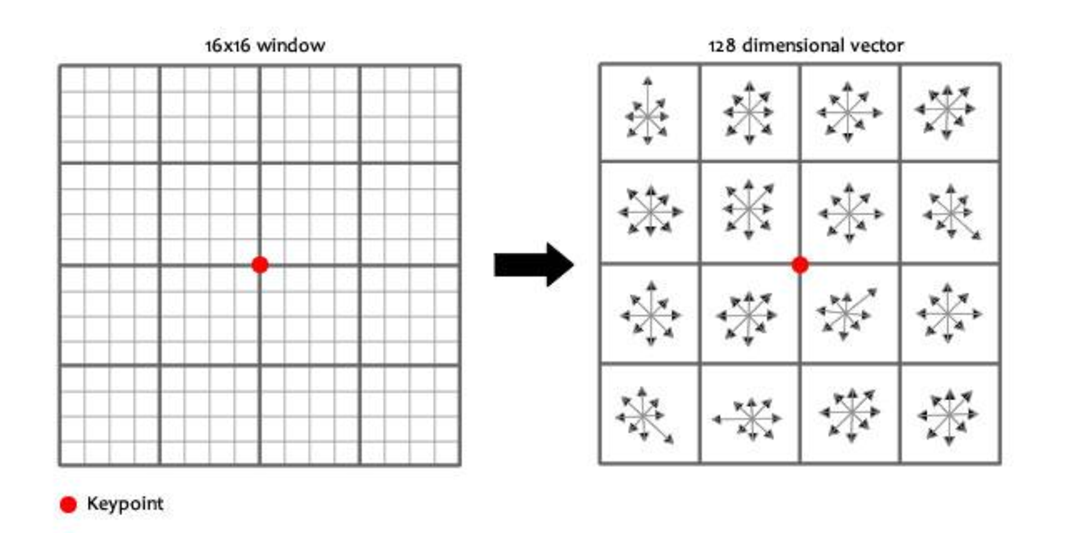
\includegraphics[width=0.9\columnwidth]{2.mainmatter/2.Methodology/FeaturesExtraction/figures/SIFT/keypoint-descriptor}%
\caption[Creation of Key-point Descriptor]{Creation of keypoint descriptor. Image gradients are used to create image descriptor. \imgsrc{(Image source: Sinha~\cite{Sinha:10:online})}}%
\label{fig:keypoint-descriptor}%
\end{figure}
\end{enumerate}
